\section{Spectrum of the BCS Hamiltonian}

\subsection{Gap Equation at Zero Temperature}

The elementary excitations over the many-body ground state \( |\psi_0\rangle \) are created by the Bogoliubov quasiparticle operators \( \gamma_{\mathbf{k},\sigma}^\dagger \). These states naturally form the eigenvectors of the diagonalized grand canonical Hamiltonian:
\[
    \hat{K}\gamma_{\mathbf{k},\sigma}^\dagger |\psi_0\rangle = (E_{\mathbf{k}} + C')\gamma_{\mathbf{k},\sigma}^\dagger |\psi_0\rangle,
\]
with the quasiparticle energy dispersion given by \( E_{\mathbf{k}} = \sqrt{\xi_k^2 + |\Delta_{\mathbf{k}}|^2} \). We are considering single quasiparticle excitations, which are the lowest-lying excited states of the system. The energy of a single quasiparticle excitation is therefore \( E_{\mathbf{k}} \) above the ground state energy \( C' \).

Consider the physical implications of this dispersion relation: whenever the momentum-dependent parameter \( \Delta_{\mathbf{k}} \neq 0 \), the excitation energy satisfies \( E_{\mathbf{k}} > 0 \) for all momenta \( \mathbf{k} \). Consequently, there exists a strictly positive energy gap between the superconducting ground state and the lowest-lying first excited state (which is determined by the global minimum of \( E_{\mathbf{k}} \)). For this fundamental reason, the function \( \Delta_{\mathbf{k}} \) is commonly referred to as the \emph{gap function}.

Recall that the gap function \( \Delta_{\mathbf{k}} \) was originally defined self-consistently through the expectation value of the pair destruction operator, \( A_{\mathbf{k}} = \langle c_{-\mathbf{k},\downarrow} c_{\mathbf{k},\uparrow} \rangle \), which looks like a self-consistency condition for the gap function: we are trying to find a solution for \( \Delta_{\mathbf{k}} \) that is consistent with the expectation value of the pair operator in the BCS ground state. The gap function is therefore determined by the microscopic details of the interaction potential \( V(\mathbf{k}, \mathbf{k}') \) and the underlying Fermi surface. Let us explicitly compute this thermodynamic average at absolute zero temperature (\( T = 0 \)), meaning we evaluate the expectation value strictly over the BCS ground state. Using the inverse Bogoliubov transformations, we express the bare particle operators in terms of the quasiparticle operators:
\[
    A_{\mathbf{k}} = \langle c_{-\mathbf{k},\downarrow} c_{\mathbf{k},\uparrow} \rangle = \left\langle \left( -v_{\mathbf{k}} \gamma_{\mathbf{k},\uparrow}^\dagger + u_{\mathbf{k}}^* \gamma_{-\mathbf{k},\downarrow} \right) \left( v_{\mathbf{k}} \gamma_{-\mathbf{k},\downarrow}^\dagger + u_{\mathbf{k}}^* \gamma_{\mathbf{k},\uparrow} \right) \right\rangle = u_{\mathbf{k}}^* v_{\mathbf{k}},
\]
where we have used the fact that \( \gamma_{\mathbf{k},\sigma} |\psi_0\rangle = 0 \). One can readily verify from the explicit definitions of the coherence factors \( u_{\mathbf{k}} \) and \( v_{\mathbf{k}} \) that their product yields:
\[
    u_{\mathbf{k}}^* v_{\mathbf{k}} = \frac{\Delta_{\mathbf{k}}}{2E_{\mathbf{k}}}.
\]
Substituting this relation back into the definition of the gap parameter, we obtain the discrete self-consistency equation:
\[
    \Delta_{\mathbf{k}} = -\frac{1}{V} \sum_{\mathbf{k}'} V(\mathbf{k}, \mathbf{k}') \frac{\Delta_{\mathbf{k}'}}{2E_{\mathbf{k}'}}.
\]
Taking the thermodynamic limit, the momentum sum transitions into an integral, yielding the celebrated BCS gap equation:
\begin{equation} \label{eq:bcs_gap_equation}
    \Delta_{\mathbf{k}} = -\int \frac{\mathrm{d}^3\mathbf{k}'}{(2\pi)^3} \frac{V(\mathbf{k}, \mathbf{k}')}{2E_{\mathbf{k}'}} \Delta_{\mathbf{k}'}.
\end{equation}
This is a non-linear integral equation for the gap function \( \Delta_{\mathbf{k}} \). Because \( E_{\mathbf{k}'} \) itself depends on \( \Delta_{\mathbf{k}'} \), it generally requires a numerical solution. However, in the physically relevant limit of weak interactions (which accurately models several conventional metallic superconductors), the gap equation can be solved analytically. This condition is realted to the many-body gap, which is essentially the \uline{energy cost to insert a single quasiparticle} into the system. We are still considering momenta in the vicinity of the Fermi surface, where the gap function is non-zero. The energy cost to insert a single quasiparticle is therefore the minimum of the dispersion \( \min_k E_{\mathbf{k}} = |\Delta_{\mathbf{k}}| \).

\subsubsection{Weak Coupling Solution for BCS Model of Interaction}

Let us first consider the effective phonon-mediated potential characteristic of a conventional superconductor. We approximate it as a separable, attractive well:
\[
    V(\mathbf{k}, \mathbf{k}') = -g w_k w_{k'},
\]
with a positive, constant coupling strength \( g = g_{e,ph}^2 > 0 \). We are implying that adding a quasiparticle to the system costs energy, and this cost is captured by this very rough mean-field approximation of the potential. The momentum dependence is captured by the step function \( w_k = \Theta(\hbar\omega_D - |\xi_k|) \), which restricts the interaction to a narrow energy shell of width \( 2\hbar\omega_D \) around the Fermi surface. Here, the kinetic energy relative to the chemical potential is \( \xi_k = \epsilon_k - \mu \). Note that the chemical potential \( \mu \) is approximately equal to the non-interacting Fermi energy \( E_F \) (the exact equality is slightly broken by the interaction, but \( \mu \simeq E_F \) holds to leading order).

To solve the integral gap equation \eqref{eq:bcs_gap_equation}, we proceed with a piecewise ansatz for the gap function that mirrors the symmetry of the potential:
\[
    \Delta_{\mathbf{k}} = \Delta_k = \Delta w_k.
\]
Substituting this ansatz and the explicit form of the interaction potential into \eqref{eq:bcs_gap_equation}, we obtain:
\[
    \Delta w_k = g \int \frac{\mathrm{d}^3\mathbf{k}'}{(2\pi)^3} \frac{w_k w_{k'} \Delta w_{k'}}{2E_{\mathbf{k}'}}.
\]
Factoring out \( \Delta w_k \) (assuming a non-trivial solution for the many body factor, \( \Delta \neq 0 \), and remembering that the dependence on \(\Delta\) is kept inside the energy denominator), the self-consistency condition simplifies to:
\[
    \frac{1}{g} = \int \frac{\mathrm{d}^3\mathbf{k}}{(2\pi)^3} \frac{\Theta(\hbar\omega_D - |\xi_k|)}{2E_k}.
\]
In the relevant region of integration specified by the Heaviside step function \( \Theta \), the quasiparticle dispersion is:
\[
    E_{\mathbf{k}} = E_k = \sqrt{\xi_k^2 + |\Delta|^2}.
\]
The minimum of this dispersion is \( \min_k E_k = |\Delta| \), which is reached exactly at the Fermi surface where \( \xi_k = 0 \) (corresponding to \( k = \sqrt{2m\mu}/\hbar \simeq k_F \)). Notice that the gap equation only dictates the modulus of the gap \( |\Delta| \), leaving the global phase undetermined. Without loss of generality, we can therefore assume \( \Delta \) to be strictly real and positive.

To evaluate the momentum integral, we transition to an energy integration for convenience by introducing the single-particle density of states \( N(\xi) \) \textit{per spin component}\footnote{We are ignoring the spin degeneracy in this discussion.} and per unit volume:
\begin{equation} \label{eq:density_of_states}
    N(\xi) = \int \frac{\mathrm{d}^3\mathbf{k}}{(2\pi)^3} \delta(\xi - \xi_k) = \frac{m^{3/2}}{\sqrt{2}\pi^2\hbar^3} \sqrt{\xi + \mu},
\end{equation}
where the last equality is obtained by explicitly evaluating the delta function integral in spherical coordinates. Physically, the density of states \( N(\xi) \) counts the number of single-particle states per unit energy interval and per unit volume. Using this definition, the gap equation transforms into:
\[
    \frac{1}{g} = \int_{-\mu}^{+\infty} d\xi \frac{N(\xi)}{2E_{\xi}} \Theta(\hbar\omega_D - |\xi|),
\]
where \( E_{\xi} = \sqrt{\xi^2 + |\Delta|^2} \), and the integral is still counting the volume of the phase space (in energy, the density of states takes the role of a weight function). Because the Debye energy is typically orders of magnitude smaller than the Fermi energy (\( \hbar\omega_D \ll E_F \approx \mu \)), the lower limit of integration \( -\mu \) can be safely replaced by the step function's cutoff \( -\hbar\omega_D \):
\[
    \frac{1}{g} = \int_{-\hbar\omega_D}^{\hbar\omega_D} d\xi \frac{N(\xi)}{2E_{\xi}}.
\]

\begin{figure}[H]
    \centering
    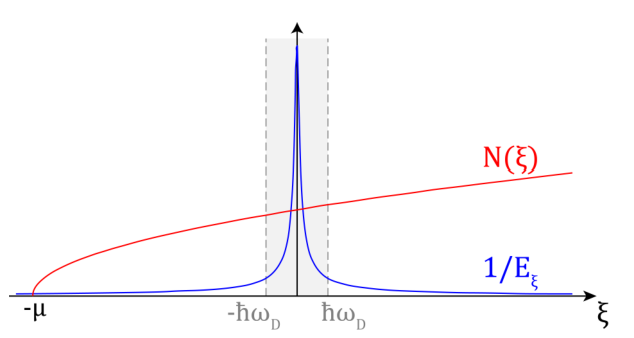
\includegraphics[width=0.8\textwidth]{img/2-bcs_density_of_states_vs_dispersion.png}
    \caption{Plot of the single-particle density of states \( N(\xi) \) and the inverse of the quasiparticle dispersion \( 1/E_\xi \), where \( E_\xi = \sqrt{\xi^2 + |\Delta|^2} \). The shaded region visually represents the narrow integration shell defined by the Debye energy cutoff \( \pm\hbar\omega_D \). Within this small window around the Fermi surface (\( \xi = 0 \)), \( 1/E_\xi \) is strongly peaked, whereas the density of states varies negligibly and can be robustly approximated by its constant value at the Fermi level, \( N_0 = N(0) \).}
    \label{fig:density_of_states_vs_dispersion}
\end{figure}

We must now carefully analyze the weak-coupling limit, where \( g \to 0 \). For the equation to hold, the right-hand side integral must correspondingly diverge towards \( +\infty \). This logarithmic divergence is only possible if the gap parameter itself vanishes, \( \Delta \to 0 \), ensuring the integrand \( 1/E_{\xi} \to \infty \) near the Fermi surface (\( \xi = 0 \)). Under these weak-coupling conditions, the function \( 1/E_{\xi} \) is extremely sharply peaked at \( \xi = 0 \) and varies rapidly over an energy scale defined by \( \Delta \) (the peak depends on the value of \( \Delta \)). Conversely, over this exact same narrow energy shell, the density of states \( N(\xi) \) is nearly constant and can be reliably approximated by its value precisely at the Fermi level, \( N_0 \equiv N(\xi=0) \). Notice that when we say \(\Delta, g \to 0\), we mean that both parameters approach zero but never actually reach it. The limit is taken in such a way that the ratio \( \Delta/g \) remains finite and well-defined.

Pulling the constant \( N_0 \) out of the integral, we evaluate the remaining expression analytically:
\[
    \frac{1}{g} = \frac{N_0}{2} \int_{-\hbar\omega_D}^{\hbar\omega_D} \frac{\mathrm{d} \xi}{\sqrt{\xi^2 + \Delta^2}} = N_0 \int_{0}^{\hbar\omega_D} \frac{1}{\Delta \sqrt{(\frac{\xi}{\Delta})^2 + 1}} \mathrm{d} \xi = N_0 \text{arcsinh}\left(\frac{\hbar\omega_D}{\Delta}\right).
\]
Inverting this relation yields:
\[
    \frac{\hbar\omega_D}{\Delta} = \sinh\left(\frac{1}{N_0 g}\right) = \frac{e^{\frac{1}{N_0 g}} - e^{-\frac{1}{N_0 g}}}{2} \sim \frac{1}{2} \exp\left(\frac{1}{N_0 g}\right),
\]
where the final asymptotic approximation relies on the behavior of \( \sinh(x) \sim e^x / 2 \) for large arguments \( x = 1/(N_0 g) \). Solving for the physical gap parameter, we obtain the seminal weak-coupling BCS result:
\begin{equation} \label{eq:bcs_gap_zero_T}
    \Delta = 2\hbar\omega_D e^{-\frac{1}{N_0 g}}.
\end{equation}

\begin{remark}
    The exponential form of \eqref{eq:bcs_gap_zero_T} carries profound physical implications. At \( T=0 \), even an infinitesimally small attractive interaction (\( g > 0 \)) is sufficient to open a finite (albeit exponentially suppressed) energy gap \( \Delta \) at the Fermi surface. Furthermore, the function \( e^{-1/(N_0 g)} \) exhibits an essential singularity at \( g=0 \). This signifies that the superconducting state cannot be reached via standard perturbative expansions starting from the non-interacting Fermi gas; the Cooper instability is a fundamentally non-perturbative phenomenon. The dimensionless parameter \( g N_0 \) acts as the effective coupling strength, which is typically quite small in conventional phonon-mediated superconductors.
\end{remark}

The fact that now we have the Debye frequency \( \omega_D \) in the prefactor of the gap equation makes this a real many-body effect. The Debye frequency is a material property that is determined by the phonon spectrum of the solid. It is not a property of the electrons themselves, but rather of the lattice vibrations, stiffness, and the speed of sound in the material (everything is then related to the mass of the ions). The fact that the gap depends on this frequency shows that the superconducting state is a collective effect that arises from the interaction between electrons and the lattice vibrations.

\subsubsection{Weak Coupling Solution for Ultracold Fermi Gases}

We now shift our focus to ultracold Fermi gases, where the effective interaction is characterized by a short-range contact potential. In momentum space, this is modeled as \( V(\mathbf{k}, \mathbf{k}') = v_0 w_k w_{k'} \), with the cutoff function \( w_k = \Theta(k_0 - k) \).\TODO{add image of omega as cutoff function} We are physically interested in the limit where the ultraviolet cutoff momentum is taken to infinity, \( k_0 \to \infty \). To ensure physical observables remain well-defined, the bare coupling strength \( v_0 \) must be simultaneously rescaled (renormalized) in order to hold the low-energy \( s \)-wave scattering length \( a \) constant.

Applying the same piecewise ansatz for the gap function, \( \Delta_{\mathbf{k}} = \Delta_k = \Delta w_k \), the generalized gap equation \eqref{eq:bcs_gap_equation} becomes:
\[
    \Delta w_k = -v_0 \int \frac{\mathrm{d}^3\mathbf{k}'}{(2\pi)^3} \frac{w_k w_{k'} \Delta w_{k'}}{2E_{k'}}.
\]
From now on we repeat the same computation done for the superconducing case. Dividing by \( \Delta w_k \) yields the bare relation:
\[
    -\frac{1}{v_0} = \int \frac{\mathrm{d}^3\mathbf{k}}{(2\pi)^3} \frac{w_k^2}{2E_k}.
\]
To eliminate the divergent bare coupling \( v_0 \) in favor of the physical scattering length \( a \), we formally add and subtract an identical free-particle integral containing the bare kinetic energy \( \epsilon_k = \hbar^2 k^2 / (2m) \):
\[
    -\frac{1}{v_0} = \int \frac{\mathrm{d}^3\mathbf{k}}{(2\pi)^3} \left( \frac{1}{2E_k} - \frac{1}{2\epsilon_k} \right) w_k^2 + \int \frac{\mathrm{d}^3\mathbf{k}}{(2\pi)^3} \frac{w_k^2}{2\epsilon_k}.
\]
We recognize that the bare coupling and the last integral term are exactly related by the Lippmann-Schwinger equation for the \( T \)-matrix at zero energy, which defines the running of \( v_0 \) with the scattering length \( a \):
\[
    -\frac{m}{4\pi\hbar^2 a} = \int \frac{\mathrm{d}^3\mathbf{k}}{(2\pi)^3} \left( \frac{1}{2E_k} - \frac{1}{2\epsilon_k} \right) w_k^2.
\]
Because the integrand in the parenthesis now scales as \( k^{-4} \) for large momenta, the integral is explicitly ultraviolet convergent. We can therefore safely remove the artificial regularization by taking the limit \( k_0 \to \infty \), yielding the fully regularized gap equation:
\begin{equation} \label{eq:ultracold_gap_regularized}
    -\frac{m}{4\pi\hbar^2 a} = \int \frac{\mathrm{d}^3\mathbf{k}}{(2\pi)^3} \left( \frac{1}{2E_k} - \frac{1}{2\epsilon_k} \right).
\end{equation}

This convergent integral can be evaluated analytically in terms of complete elliptic integrals. Let us consider the specific regime of a weak attractive interaction, characterized by a small and negative scattering length \( a \to 0^- \). In this BCS-like limit, the chemical potential approaches the non-interacting Fermi energy (\( \mu \simeq E_F \)) and the gap is small (\( \Delta \ll \mu \)). The regularized integration yields the explicit asymptotic solution:
\begin{equation} \label{eq:ultracold_gap_result}
    \Delta = \frac{8E_F}{e^2} e^{\frac{\pi}{2 k_F a}}.
\end{equation}
This profound result explicitly dictates how the pairing gap becomes exponentially suppressed in the limit \( k_F a \to 0^- \). Physically, adding particles to the system costs energy, and this cost is captured by this very rough mean-field approximation of the potential. The gap is exponentially small in the weak-coupling limit, but it is non-zero for any finite attractive interaction, indicating that the system is unstable.

It is structurally insightful to compare this ultracold gas result with the solid-state BCS expression \eqref{eq:bcs_gap_zero_T}. Recall that the 3D density of states at the Fermi surface is \( N_0 = (m k_F)/(2\pi^2\hbar^2) \). If we identify the effective BCS coupling parameter with the first-order Born approximation of the scattering amplitude, \( g = -4\pi\hbar^2 a / m \), the exponential dependence \( e^{\pi/(2 k_F a)} \) strictly coincides with the BCS term \( e^{-1/(N_0 g)} \). This mapping perfectly reproduces the exponent; however, retaining the full \( 1/(2\epsilon_k) \) counter-term in the integral regularization—rather than relying strictly on the lowest-order Born approximation—is mathematically critical for capturing the exact \( 8/e^2 \) numerical prefactor governing the overall energy scale of the pairing gap.

\subsubsection{Comparison with Spectrum of the Weak Interacting Bose Gas}

In the case of a weakly interacting Bose gas, the spectrum of elementary excitations is determined by the Bogoliubov dispersion relation:...\TODO{complete, graph and compare}

[drawing of ``BCS wavefunction'' as a product of pairs of fermions in momentum space, with arrows indicating the pairing of opposite momenta and spins]

In order to create an excitation, we have to add momenta to an electron inside a cooper pair, but this cannot be done continuously because the two electrons are bound together. The energy cost to break a pair is the gap \( \Delta \). In contrast, in a weakly interacting Bose gas, the Bogoliubov spectrum is gapless, and excitations can be created with arbitrarily small energy by adding small momenta to the condensate. This fundamental difference in the excitation spectrum leads to distinct physical properties between fermionic superfluids and bosonic condensates.

the cooper pairs can be broke releasing energy or absorbing energy interacting with the phonons (we have ignored them for a while but they are still in the description).

transition to the landau criterion...

















\subsection{Elementary Excitations and Landau Criterion}

All the excited states of the grand-canonical Hamiltonian \( \hat{K} \) are systematically obtained by acting with the quasiparticle creation operator \( \gamma_{\mathbf{k},\sigma}^\dagger \) on the many-body ground state \( |\psi_0(\mu)\rangle \). The energy dispersion of these elementary excitations in a BCS superconductor or superfluid is thus given by \( E_k = \sqrt{\xi_k^2 + |\Delta|^2} \).

To fully appreciate the physical consequences of the Bogoliubov quasiparticle spectrum derived from the zero-temperature gap equation, it is highly instructive to compare the dispersion profile \( \varepsilon = E_{\mathbf{k}} \) as a function of the momentum magnitude \( k = |\mathbf{k}| \) for a Weakly Interacting Bose Gas (WIBG) against that of a BCS superconductor:
\begin{itemize}
    \item \textbf{Weakly Interacting Bose Gas (WIBG):} Via the bosonic Bogoliubov transformation, the elementary excitations are created by the bosonic quasiparticle operators \( \alpha_{\mathbf{k}}^\dagger \) and follow the gapless dispersion relation:
          \[
              E_{\mathbf{k}}^{\text{WIBG}} = \sqrt{(\epsilon_{\mathbf{k}} + nU_0)^2 - (nU_0)^2} = \sqrt{\epsilon_{\mathbf{k}}^2 + 2nU_0\epsilon_{\mathbf{k}}},
          \]
          which vanishes linearly as \( E_{\mathbf{k}}^{\text{WIBG}} \simeq c\hbar k \) in the long-wavelength limit (\( k \to 0 \), representing the phononic Goldstone mode with sound velocity \( c = \sqrt{nU_0/m} \)) and smoothly crosses over to the quadratic free-particle behavior \( \epsilon_{\mathbf{k}} + nU_0 \sim \frac{\hbar^2 k^2}{2m} \) at large momenta.
    \item \textbf{BCS Superconductor:} By contrast, in a BCS superconductor the elementary excitations are created by the fermionic Bogoliubov quasiparticle operators \( \gamma_{\mathbf{k},\sigma}^\dagger \) and are governed by the strictly gapped dispersion:
          \[
              E_{\mathbf{k}}^{\text{BCS}} = \sqrt{\xi_{\mathbf{k}}^2 + |\Delta_{\mathbf{k}}|^2}, \quad \text{with} \quad \xi_{\mathbf{k}} = \epsilon_{\mathbf{k}} - \mu.
          \]
          At \( k = 0 \), the excitation energy starts at a finite value. Taking into account the momentum profile of the gap around the active energy shell, the dispersion exhibits a characteristic non-monotonic shape that reaches its absolute minimum \( \Delta \) at a finite momentum \( k_{\text{min}} \neq 0 \) (located precisely at the Fermi surface \( k_{\text{min}} \simeq k_F \), where \( \xi_{\mathbf{k}} = 0 \) and the phonon-mediated attractive interaction within the Debye window \( \hbar\omega_D \) is active), before growing quadratically at large momenta (\( k \gg k_{\text{min}} \)). In order to create a single-particle excitation, one must impart momentum to an electron bound within a Cooper pair; this process cannot occur continuously from zero energy because the pair is bound together, requiring a minimum threshold energy of \( \Delta \) (or \( 2\Delta \) to break a pair into two quasiparticles) via the absorption or emission of lattice phonons.
\end{itemize}

\TODO{add image of a comparison plot between the elementary excitation spectrum of a weakly interacting Bose gas and a BCS superconductor showing the linear bounding slope from the origin for the Landau critical velocity}

By applying \textbf{Landau's criterion for superfluidity} to this specific dispersion relation \( E_{\mathbf{k}} \), we look geometrically for the minimum of the ratio \( E_k / (\hbar k) \). Because the excitation spectrum is strictly gapped around \( k_{\text{min}} \neq 0 \), the straight line starting from the origin and tangent to the minimum of the dispersion curve possesses a strictly positive slope:
\[
    v_c = \min_{\mathbf{k}} \frac{E_{\mathbf{k}}}{\hbar k} \simeq \frac{\Delta}{\hbar k_F} > 0,
\]
which holds in the physically relevant regime where \( \Delta \ll E_F \). For flow velocities below \( v_c \), no elementary excitations can be kinematically nucleated, and the system supports dissipationless flow without friction. In a charged system, this directly translates into the complete vanishing of electrical resistivity (\( \rho = 0 \)) below the critical temperature \( T_c \), contrasting sharply with the normal metallic state where resistivity remains finite and typically scales as \( T^3 \) (or \( T^5 \) in the standard Bloch-Grüneisen electron-phonon regime) at low temperatures before dropping abruptly to zero at the superconducting transition. We thus arrive at the striking physical conclusion that BCS theory combined with the Landau kinematic criterion rigorously predicts that an attractively interacting Fermi gas fundamentally behaves as a superfluid (if neutral) or a superconductor (if charged) at \( T = 0 \): \emph{superconductors are superfluids of Cooper pairs}.

\subsubsection{Comparison of Ground-State Wave Functions and the Role of Quantum Statistics}

To truly appreciate what it means for a superconductor to behave as a superfluid of Cooper pairs, we must address a subtle and seemingly counterintuitive question regarding the quantum statistics of the underlying pairs. Let us compare the explicit algebraic structure of the ground-state wave function of a BCS superconductor with that of a Weakly Interacting Bose Gas:
\begin{enumerate}
    \item \textbf{BCS Ground-State Wave Function:} Introducing the Cooper-pair creation operator \( D_{\mathbf{k}}^\dagger = c_{\mathbf{k},\uparrow}^\dagger c_{-\mathbf{k},\downarrow}^\dagger \), which creates a pair of fermions with opposite momenta and opposite spins \( (\mathbf{k}\uparrow, -\mathbf{k}\downarrow) \), the variational BCS ground state reads:
          \begin{equation} \label{eq:bcs_ground_state_pair_operator}
              |\Psi_{\text{BCS}}\rangle = \prod_{\mathbf{k}} \left( A_{\mathbf{k}} + B_{\mathbf{k}} D_{\mathbf{k}}^\dagger \right) |0\rangle, \quad \text{where} \quad \left( D_{\mathbf{k}}^\dagger \right)^2 = 0,
          \end{equation}
          with variational coherence coefficients \( A_{\mathbf{k}} = u_{\mathbf{k}} \) and \( B_{\mathbf{k}} = v_{\mathbf{k}} \) normalized such that \( |u_{\mathbf{k}}|^2 + |v_{\mathbf{k}}|^2 = 1 \). Crucially, because the constituent particles are fermions obeying canonical anticommutation relations \( \{c_{\mathbf{k},\sigma}^\dagger, c_{\mathbf{k}',\sigma'}^\dagger\} = 0 \), the pair creation operator is strictly \textbf{nilpotent}:
          \[
              \left( D_{\mathbf{k}}^\dagger \right)^2 = c_{\mathbf{k},\uparrow}^\dagger c_{-\mathbf{k},\downarrow}^\dagger c_{\mathbf{k},\uparrow}^\dagger c_{-\mathbf{k},\downarrow}^\dagger = - \left( c_{\mathbf{k},\uparrow}^\dagger \right)^2 \left( c_{-\mathbf{k},\downarrow}^\dagger \right)^2 = 0.
          \]
          Physically, the Pauli exclusion principle strictly forbids placing two identical fermions—and hence two Cooper pairs with the exact same relative momentum \( \mathbf{k} \)—into the same single-particle quantum state.
    \item \textbf{Weakly Interacting Bose Gas (WIBG) Ground-State Wave Function:} By contrast, recall how the ground state of a Weakly Interacting Bose Gas is constructed in terms of the elementary bosonic creation operators \( a_{\mathbf{k}}^\dagger \). Its coherent-like structure over the momentum modes is summarized schematically as \( |\Psi_{\text{WIBG}}\rangle = \prod_{\mathbf{k}} e^{\alpha a_{\mathbf{k}}^\dagger} |0\rangle \), which encapsulates the exact Bogoliubov ground-state wave function combining the coherent state for the \( \mathbf{k} = \mathbf{0} \) condensate mode with the exponential of bosonic pair creation operators for \( \mathbf{k} \neq \mathbf{0} \):
          \[
              |\Psi_{\text{WIBG}}\rangle = \frac{1}{\mathcal{N}} e^{\sqrt{N_0} a_{\mathbf{0}}^\dagger} \exp\left( -\frac{1}{2} \sum_{\mathbf{k} \neq \mathbf{0}} \frac{v_{\mathbf{k}}}{u_{\mathbf{k}}} a_{\mathbf{k}}^\dagger a_{-\mathbf{k}}^\dagger \right) |0\rangle = \frac{1}{\mathcal{N}} e^{\sqrt{N_0} a_{\mathbf{0}}^\dagger} \prod_{\mathbf{k} \neq \mathbf{0}} \exp\left( -\frac{1}{2} \frac{v_{\mathbf{k}}}{u_{\mathbf{k}}} a_{\mathbf{k}}^\dagger a_{-\mathbf{k}}^\dagger \right) |0\rangle.
          \]
\end{enumerate}

Comparing the operators generating the two ground states highlights a fundamental algebraic distinction between Cooper pairs and true elementary bosons:
\[
    \left( D_{\mathbf{k}}^\dagger \right)^2 = 0 \quad \longleftrightarrow \quad a_{\mathbf{k}}^2 \neq 0 \quad \left( \text{and } (a_{\mathbf{k}}^\dagger)^2 \neq 0 \right).
\]
In a Bose gas, the operators \( a_{\mathbf{k}}^\dagger \) (as well as the bosonic pair operators \( a_{\mathbf{k}}^\dagger a_{-\mathbf{k}}^\dagger \)) can be applied an arbitrary number of times \( n \) to the vacuum without vanishing, generating all higher-order terms \( \frac{1}{n!} (a_{\mathbf{k}}^\dagger)^n \) in the Taylor expansion of the exponential. In a BCS superconductor, instead, the hard-core fermionic constraint \( (D_{\mathbf{k}}^\dagger)^2 = 0 \) truncates the exponential series \( \exp\left( \frac{v_{\mathbf{k}}}{u_{\mathbf{k}}} D_{\mathbf{k}}^\dagger \right) = 1 + \frac{v_{\mathbf{k}}}{u_{\mathbf{k}}} D_{\mathbf{k}}^\dagger \) at first order, meaning that a given \( (\mathbf{k}\uparrow, -\mathbf{k}\downarrow) \) mode can accommodate at most one Cooper pair.

Given that \( (D_{\mathbf{k}}^\dagger)^2 = 0 \) prevents multiple occupation of the same relative momentum state, a natural question arises: \emph{How can we legitimately invoke Landau's criterion—which was originally derived for a Bose gas—to conclude that a BCS superconductor is a superfluid of Cooper pairs?} The resolution of this apparent paradox lies in a fundamental physical principle: \textbf{Landau's criterion does not care about quantum statistics; it is based exclusively on the excitation spectrum and energetics}. To see why rigorously, let us recall how Landau's criterion is constructed:
\begin{itemize}
    \item \textbf{Single-Excitation Energetics:} In the reference frame moving with the fluid, the system starts in its many-body ground state \( |\Psi_0\rangle \) with energy \( \mathcal{E}_0 \). To determine the onset of dissipation (friction), Landau's kinematic argument simply asks whether it is energetically favorable to create a \emph{single extra elementary excitation} of momentum \( \hbar\mathbf{k} \) and energy \( E_{\mathbf{k}} \), which shifts the energy in the laboratory frame by \( \Delta E = E_{\mathbf{k}} + \hbar\mathbf{k} \cdot \mathbf{v} \).
    \item \textbf{Indistinguishability of Statistics for a Single Quasiparticle:} In the Weakly Interacting Bose Gas, creating a single elementary excitation above the ground state corresponds to acting once with the bosonic Bogoliubov operator \( \alpha_{\mathbf{k}}^\dagger |\Psi_{\text{WIBG}}\rangle \). In the BCS superconductor, creating a single elementary excitation corresponds to acting once with the fermionic Bogoliubov quasiparticle operator \( \gamma_{\mathbf{k},\sigma}^\dagger |\Psi_{\text{BCS}}\rangle \). As long as we consider the creation of a \textbf{single excitation} (one quasiparticle), it is physically and mathematically impossible to distinguish whether that single excitation obeys bosonic or fermionic statistics.
    \item \textbf{When Would Statistics Matter?} Quantum statistics (Fermi-Dirac versus Bose-Einstein, or Pauli blocking) only manifests itself when we attempt to populate \emph{multiple} particles or excitations in the exact same quantum state. If the stability criterion for superfluidity had required the simultaneous creation of a macroscopic multiparticle state in a single mode, statistics would have played a decisive role. However, because the threshold for dissipation is governed entirely by the kinematic cost of nucleating the \emph{first} single elementary excitation, Landau's criterion depends exclusively on the single-quasiparticle dispersion relation \( E_{\mathbf{k}} \) (purely energetics), remaining completely blind to the underlying quantum statistics.
\end{itemize}

\subsubsection{Momentum Distribution Function}

The average number of fermions with momentum \( \mathbf{k} \) and spin \( \sigma \) in the ground state \( |\psi_0\rangle \) (at \( T = 0 \)) is defined by the expectation value of the bare number operator:
\[
    n_{\mathbf{k},\sigma} = \langle c_{\mathbf{k},\sigma}^\dagger c_{\mathbf{k},\sigma} \rangle.
\]
Experimentally, this quantity can be probed directly in ultracold atomic gases via time-of-flight (TOF) expansion measurements: when the trapping potential is abruptly switched off, the gas expands freely, and in the ballistic regime the final spatial positions of the independent atoms map directly onto their initial momenta, rendering the imaged spatial density profile directly proportional to the momentum distribution \( n_{\mathbf{k},\sigma} \). For an ideal non-interacting Fermi gas at \( T = 0 \), this distribution is a sharp Heaviside step function \( \Theta(k_F - k) \); in the interacting BCS state, we expect to recover this exact step behavior everywhere outside the narrow energy shell surrounding the Fermi surface, within which the emergent many-body pairing correlations will smear the distribution.

To evaluate \( n_{\mathbf{k},\sigma} \) analytically, we utilize the inverse Bogoliubov transformations, which explicitly dictate the relations between the bare particle operators \( c_{\mathbf{k},\sigma}, c_{\mathbf{k},\sigma}^\dagger \) and the Bogoliubov quasiparticle operators \( \gamma_{\mathbf{k},\sigma}, \gamma_{\mathbf{k},\sigma}^\dagger \):
\[
    c_{\mathbf{k},\uparrow} = u_{\mathbf{k}}^* \gamma_{\mathbf{k},\uparrow} + v_{\mathbf{k}} \gamma_{-\mathbf{k},\downarrow}^\dagger, \quad c_{\mathbf{k},\downarrow} = u_{\mathbf{k}}^* \gamma_{\mathbf{k},\downarrow} - v_{\mathbf{k}} \gamma_{-\mathbf{k},\uparrow}^\dagger.
\]
Taking the Hermitian conjugate yields the corresponding creation operators:
\[
    c_{\mathbf{k},\uparrow}^\dagger = u_{\mathbf{k}} \gamma_{\mathbf{k},\uparrow}^\dagger + v_{\mathbf{k}}^* \gamma_{-\mathbf{k},\downarrow}, \quad c_{\mathbf{k},\downarrow}^\dagger = u_{\mathbf{k}} \gamma_{\mathbf{k},\downarrow}^\dagger - v_{\mathbf{k}}^* \gamma_{-\mathbf{k},\uparrow}.
\]
Because the BCS ground state is defined as the quasiparticle vacuum (\( \gamma_{\mathbf{k},\sigma} |\psi_0\rangle = 0 \)), only the terms involving anti-normal-ordered quasiparticle operators \( \gamma \gamma^\dagger \) contribute to the expectation value. We thus obtain:
\[
    \langle c_{\mathbf{k},\uparrow}^\dagger c_{\mathbf{k},\uparrow} \rangle = \langle v_{\mathbf{k}}^* v_{\mathbf{k}} \gamma_{-\mathbf{k},\downarrow} \gamma_{-\mathbf{k},\downarrow}^\dagger \rangle = |v_{\mathbf{k}}|^2, \quad \langle c_{\mathbf{k},\downarrow}^\dagger c_{\mathbf{k},\downarrow} \rangle = \langle (-v_{\mathbf{k}}^*)(-v_{\mathbf{k}}) \gamma_{-\mathbf{k},\uparrow} \gamma_{-\mathbf{k},\uparrow}^\dagger \rangle = |v_{\mathbf{k}}|^2.
\]
Recalling the explicit analytical expression for the coherence factor \( v_{\mathbf{k}} \), one obtains the ground-state momentum distribution:
\begin{equation} \label{eq:momentum_distribution}
    n_{\mathbf{k},\sigma} = |v_{\mathbf{k}}|^2 = \frac{1}{2} \left( 1 - \frac{\xi_k}{E_k} \right).
\end{equation}

\TODO{add image of a plot showing the momentum distribution function as a function of momentum displaying a smeared Fermi step near the Fermi momentum compared to the sharp step of a non interacting Fermi gas}

In the weak-coupling regime where \( \Delta \ll E_F \), the pairing gap is much smaller than the relative kinetic energy \( |\xi_k| \), except within a very narrow momentum window of width \( \delta k \sim (m\Delta)/(\hbar^2 k_F) \) centered directly around the Fermi momentum \( k_F \). Outside this specific window, the dispersion smoothly approximates the absolute value of the kinetic energy, \( E_k = \sqrt{\xi_k^2 + |\Delta|^2} \approx |\xi_k| \). Consequently, the distribution sharply approaches \( n_{\mathbf{k},\sigma} \simeq 1 \) for states deep inside the Fermi sea (\( \xi_k < 0 \)), or \( n_{\mathbf{k},\sigma} \simeq 0 \) for states far above it (\( \xi_k > 0 \)). One thus naturally recovers a momentum distribution that essentially coincides with the standard Heaviside step distribution of an ideal non-interacting Fermi gas at \( T = 0 \), with the crucial modification of a continuous smearing confined to a small momentum window around \( k_F \) whose width is governed directly by the magnitude of the pairing gap \( \Delta \).

\subsection{Gap Equation at Finite Temperature}

At absolute zero temperature (\( T = 0 \)), the system resides in a pure quantum state—the BCS ground state \( |\psi_0\rangle \)—and the anomalous Cooper-pair amplitude \( \langle c_{-\mathbf{k},\downarrow} c_{\mathbf{k},\uparrow} \rangle \) entering the gap function \( \Delta_{\mathbf{k}} \) was evaluated using the vacuum property \( \gamma_{\mathbf{k},\sigma} |\psi_0\rangle = 0 \), which implies \( \langle \gamma_{\mathbf{k},\sigma}^\dagger \gamma_{\mathbf{k},\sigma} \rangle = 0 \).

At any finite temperature (\( T > 0 \)), we can no longer evaluate expectation values over a single pure wave function because thermal fluctuations excite the system into a \textbf{statistical mixed state}. Consequently, pure ground-state averages must be rigorously replaced by thermal averages computed via the grand-canonical density matrix:
\[
    \langle \hat{O} \rangle = \frac{\text{Tr}\left( e^{-\beta \hat{K}} \hat{O} \right)}{\mathcal{Z}}, \quad \text{with} \quad \mathcal{Z} = \text{Tr}\left( e^{-\beta \hat{K}} \right).
\]
To characterize this mixed state for \( T > 0 \), recall that our diagonalized grand-canonical Hamiltonian operator \( \hat{K} = \hat{H} - \mu \hat{N} \) takes the form:
\[
    \hat{K} = \sum_{\mathbf{k},\sigma} E_{\mathbf{k}} \gamma_{\mathbf{k},\sigma}^\dagger \gamma_{\mathbf{k},\sigma} + C',
\]
where the scalar constant offset \( C' \) identically cancels out between the numerator and denominator in thermal averages, leaving the effective operator \( \hat{K}' = \sum_{\mathbf{k},\sigma} E_{\mathbf{k}} \gamma_{\mathbf{k},\sigma}^\dagger \gamma_{\mathbf{k},\sigma} \).

\begin{remark}
    Notice that \( \hat{K}' \) formally describes a gas of \textbf{independent, non-interacting fermionic quasiparticles}, coinciding structurally with the Hamiltonian of an ideal Fermi gas, with the critical distinction that the bare single-particle dispersion \( \xi_k = \epsilon_k - \mu \) is replaced by the superconducting quasiparticle dispersion \( E_{\mathbf{k}} = \sqrt{\xi_{\mathbf{k}}^2 + |\Delta_{\mathbf{k}}|^2} \).
\end{remark}

With this direct structural identification, we conclude immediately that in the thermal mixed state at \( T > 0 \), the average occupation of the fermionic quasiparticle modes is governed by the standard \textbf{Fermi-Dirac distribution}:
\[
    \langle \gamma_{\mathbf{k},\sigma}^\dagger \gamma_{\mathbf{k},\sigma} \rangle = f(E_{\mathbf{k}}) = \frac{1}{e^{\beta E_{\mathbf{k}}} + 1},
\]
where \( \beta = 1/(k_B T) \), and \( f(E_{\mathbf{k}}) \) is independent of the spin index \( \sigma \) because the dispersion \( E_{\mathbf{k}} \) is spin-independent. Notice that this relation holds in any spatial dimension; at any finite temperature \( T > 0 \), every quasiparticle state of arbitrary energy \( E_{\mathbf{k}} \) acquires a small but strictly non-zero thermal occupation.

\subsubsection{Evaluation of the Finite-Temperature Anomalous Pairing Average}

We now re-evaluate the thermal expectation value of the anomalous Cooper-pair operator at finite temperature by expressing the bare fermionic operators in terms of the Bogoliubov quasiparticle operators via the inverse Bogoliubov transformation:
\[
    \langle c_{-\mathbf{k},\downarrow} c_{\mathbf{k},\uparrow} \rangle = \left\langle \left( -v_{\mathbf{k}} \gamma_{\mathbf{k},\uparrow}^\dagger + u_{\mathbf{k}}^* \gamma_{-\mathbf{k},\downarrow} \right) \left( u_{\mathbf{k}}^* \gamma_{\mathbf{k},\uparrow} + v_{\mathbf{k}} \gamma_{-\mathbf{k},\downarrow}^\dagger \right) \right\rangle.
\]
(Note that since the global phase can be chosen such that \( \Delta_{\mathbf{k}} \) and the coherence factors \( u_{\mathbf{k}}, v_{\mathbf{k}} \) are real, the expectation values \( \langle c_{-\mathbf{k},\downarrow} c_{\mathbf{k},\uparrow} \rangle = A_{\mathbf{k}} \) and \( \langle c_{\mathbf{k},\uparrow}^\dagger c_{-\mathbf{k},\downarrow}^\dagger \rangle = A_{\mathbf{k}}^* \) coincide.) Expanding the product, the off-diagonal cross terms \( \langle \gamma_{\mathbf{k},\uparrow}^\dagger \gamma_{-\mathbf{k},\downarrow}^\dagger \rangle \) and \( \langle \gamma_{-\mathbf{k},\downarrow} \gamma_{\mathbf{k},\uparrow} \rangle \) vanish identically because the diagonal thermal density matrix \( e^{-\beta \hat{K}'} \) strictly conserves the quasiparticle number. Using the canonical fermionic anticommutation relation \( \langle \gamma_{-\mathbf{k},\downarrow} \gamma_{-\mathbf{k},\downarrow}^\dagger \rangle = 1 - \langle \gamma_{-\mathbf{k},\downarrow}^\dagger \gamma_{-\mathbf{k},\downarrow} \rangle = 1 - f(E_{\mathbf{k}}) \), we obtain step by step:
\[
    \begin{aligned}
        \langle c_{-\mathbf{k},\downarrow} c_{\mathbf{k},\uparrow} \rangle & = -v_{\mathbf{k}} u_{\mathbf{k}}^* \langle \gamma_{\mathbf{k},\uparrow}^\dagger \gamma_{\mathbf{k},\uparrow} \rangle + u_{\mathbf{k}}^* v_{\mathbf{k}} \langle \gamma_{-\mathbf{k},\downarrow} \gamma_{-\mathbf{k},\downarrow}^\dagger \rangle                                                                                           \\
                                                                           & = -v_{\mathbf{k}} u_{\mathbf{k}}^* f(E_{\mathbf{k}}) + u_{\mathbf{k}}^* v_{\mathbf{k}} [1 - f(E_{\mathbf{k}})]                                                                                                                                                                                                                           \\
                                                                           & = u_{\mathbf{k}}^* v_{\mathbf{k}} [1 - 2f(E_{\mathbf{k}})]                                                                                                                                                                                                                                                                               \\
                                                                           & = u_{\mathbf{k}}^* v_{\mathbf{k}} \left( 1 - \frac{2}{e^{\beta E_{\mathbf{k}}} + 1} \right) = u_{\mathbf{k}}^* v_{\mathbf{k}} \left( \frac{e^{\beta E_{\mathbf{k}}} - 1}{e^{\beta E_{\mathbf{k}}} + 1} \right)                                                                                                                           \\
                                                                           & = u_{\mathbf{k}}^* v_{\mathbf{k}} \left( \frac{e^{\beta E_{\mathbf{k}} / 2} - e^{-\beta E_{\mathbf{k}} / 2}}{e^{\beta E_{\mathbf{k}} / 2} + e^{-\beta E_{\mathbf{k}} / 2}} \right) \frac{e^{\beta E_{\mathbf{k}} / 2}}{e^{\beta E_{\mathbf{k}} / 2}} = u_{\mathbf{k}}^* v_{\mathbf{k}} \tanh\left(\frac{\beta E_{\mathbf{k}}}{2}\right).
    \end{aligned}
\]

\TODO{add image of a plot showing the profile of the thermal hyperbolic tangent factor as a function of inverse temperature}

Let us verify the physical consistency of this thermal factor across the two opposite temperature limits:
\begin{itemize}
    \item \textbf{Zero-Temperature Limit (\( T \to 0, \beta \to \infty \)):} In this asymptotic regime, \( \tanh\left(\frac{\beta E_{\mathbf{k}}}{2}\right) \xrightarrow{\beta \to \infty} 1 \), which smoothly recovers the exact zero-temperature BCS ground-state expectation value \( \langle c_{-\mathbf{k},\downarrow} c_{\mathbf{k},\uparrow} \rangle \xrightarrow{T \to 0} u_{\mathbf{k}}^* v_{\mathbf{k}} = \frac{\Delta_{\mathbf{k}}}{2E_{\mathbf{k}}} \).
    \item \textbf{High-Temperature Limit (\( T \to \infty, \beta \to 0 \)):} Conversely, at extreme temperatures, \( \tanh\left(\frac{\beta E_{\mathbf{k}}}{2}\right) \xrightarrow{\beta \to 0} 0 \), causing the pairing amplitude to vanish: \( \langle c_{-\mathbf{k},\downarrow} c_{\mathbf{k},\uparrow} \rangle \xrightarrow{T \to \infty} 0 \). Physically, when thermal fluctuations \( k_B T \) far exceed the pairing gap protecting the Cooper pairs, all quasiparticle states become equally populated and destructive interference completely wipes out the pairing amplitude (in fact, the superconducting phase and the mean-field description break down well before \( \beta \to 0 \), as the gap already vanishes continuously at the critical temperature \( T = T_c \)).
\end{itemize}

\subsubsection{Self-Consistent BCS Gap Equation at Finite Temperature and Low-Temperature Expansion}

By inserting the finite-temperature pairing amplitude \( \langle c_{-\mathbf{k},\downarrow} c_{\mathbf{k},\uparrow} \rangle = \frac{\Delta_{\mathbf{k}}}{2E_{\mathbf{k}}} \tanh\left(\frac{\beta E_{\mathbf{k}}}{2}\right) \) back into the fundamental self-consistent definition of the gap parameter and taking the thermodynamic continuum limit, the zero-temperature BCS gap equation is modified solely by the insertion of the hyperbolic tangent factor inside the momentum integral:
\begin{equation} \label{eq:finite_t_gap_equation}
    \Delta_{\mathbf{k}} = -\int \frac{\mathrm{d}^3\mathbf{k}'}{(2\pi)^3} \frac{V(\mathbf{k}, \mathbf{k}')}{2E_{\mathbf{k}'}} \tanh\left(\frac{\beta E_{\mathbf{k}'}}{2}\right) \Delta_{\mathbf{k}'}.
\end{equation}

Specializing to the case of a conventional superconductor governed by the separable BCS model interaction \( V_{\mathbf{k},\mathbf{k}'} = -g w_{\mathbf{k}} w_{\mathbf{k}'} \) with \( \Delta_{\mathbf{k}} = \Delta w_{\mathbf{k}} \) and \( w_{\mathbf{k}} = \Theta(\hbar\omega_D - |\xi_{\mathbf{k}}|) \), we pass from momentum integration to energy integration over \( \xi = \epsilon_{\mathbf{k}} - \mu \) via the single-particle density of states \( N(\xi) \), where \( E_\xi = \sqrt{\xi^2 + \Delta^2} \):
\[
    \frac{1}{g} = \int_{-\hbar\omega_D}^{\hbar\omega_D} \mathrm{d}\xi \frac{N(\xi)}{2E_\xi} \tanh\left(\frac{\beta E_\xi}{2}\right).
\]
Close to the Fermi energy \( E_F \) (an approximation that holds robustly in the weak-coupling regime where \( \Delta \ll E_F \) and \( T \ll T_c \ll T_F \)), the density of states can be approximated as constant across the narrow Debye shell, \( N(\xi) \simeq N_0 = N(0) \), and by exploiting the even symmetry of the integrand (\( \xi \leftrightarrow -\xi \)) we obtain:
\[
    \frac{1}{g} = N_0 \int_{0}^{\hbar\omega_D} \mathrm{d}\xi \frac{1}{E_\xi} \tanh\left(\frac{\beta E_\xi}{2}\right).
\]

Unlike the \( T = 0 \) case—where the integral reduced to \( \int_0^{\hbar\omega_D} \frac{\mathrm{d}\xi}{\sqrt{\xi^2 + \Delta^2}} = \text{arcsinh}\left(\frac{\hbar\omega_D}{\Delta}\right) \) and could be inverted analytically—the presence of the thermal factor \( \tanh\left(\frac{\beta\sqrt{\xi^2 + \Delta^2}}{2}\right) \) prevents a closed-form analytical solution for arbitrary \( T \), requiring numerical evaluation in general. However, we can derive an explicit analytical solution in the \textbf{low-temperature limit} (\( k_B T \ll \Delta_0 \), i.e., large \( \beta \to \infty \)):
\begin{itemize}
    \item \textbf{Heuristic Dimensional Estimate:} To illustrate the structure of the subleading thermal integral from a rough dimensional-analysis perspective, one might initially consider a schematic algebraic expansion of the form:
          \[
              \tanh\left(\frac{\beta E_{\mathbf{k}}}{2}\right) \simeq 1 - \left(\frac{\beta E_{\mathbf{k}}}{2}\right)^{-1} + \dots \implies \frac{1}{gN_0} = \int_0^{\hbar\omega_D} \mathrm{d}\xi \left[ \frac{1}{\sqrt{\xi^2 + \Delta^2}} - \frac{2k_B T}{\xi^2 + \Delta^2} \right] + \dots
          \]
    \item \textbf{Exact Asymptotic Expansion for \( \beta E_\xi \gg 1 \):} Rigorously, however, for large arguments \( x = \frac{\beta E_\xi}{2} \to \infty \), the exact asymptotic expansion of the hyperbolic tangent is governed by an exponential tail rather than a power law: \( \tanh(x) = \frac{1 - e^{-2x}}{1 + e^{-2x}} \simeq 1 - 2e^{-2x} = 1 - 2e^{-\beta E_\xi} \). Substituting this exact expansion into the gap equation yields:
          \[
              \frac{1}{gN_0} = \int_0^{\hbar\omega_D} \frac{\mathrm{d}\xi}{\sqrt{\xi^2 + \Delta(T)^2}} - 2 \int_0^{\hbar\omega_D} \mathrm{d}\xi \frac{e^{-\beta\sqrt{\xi^2 + \Delta(T)^2}}}{\sqrt{\xi^2 + \Delta(T)^2}}.
          \]
          Using the zero-temperature relation \( \Delta_0 = 2\hbar\omega_D e^{-1/(gN_0)} \), the first integral evaluates to \( \text{arcsinh}\left(\frac{\hbar\omega_D}{\Delta(T)}\right) \simeq \ln\left(\frac{2\hbar\omega_D}{\Delta(T)}\right) = \frac{1}{gN_0} + \ln\left(\frac{\Delta_0}{\Delta(T)}\right) \). In the second integral, because the integrand is exponentially suppressed for \( \xi \gg \sqrt{\Delta_0 k_B T} \), we can safely extend the upper integration limit to \( \infty \) and expand the dispersion as \( E_\xi \simeq \Delta_0 + \frac{\xi^2}{2\Delta_0} \) in the exponent while setting \( E_\xi \simeq \Delta_0 \) in the denominator. This reduces the thermal correction to a standard Gaussian integral:
          \[
              2 \frac{e^{-\beta\Delta_0}}{\Delta_0} \int_0^\infty \mathrm{d}\xi \, e^{-\frac{\beta\xi^2}{2\Delta_0}} = \left( \frac{2\pi k_B T}{\Delta_0} \right)^{1/2} e^{-\frac{\Delta_0}{k_B T}}.
          \]
\end{itemize}
Equating the terms and expanding the logarithm for small thermal deviations, \( \ln\left(\frac{\Delta(T)}{\Delta_0}\right) \simeq \frac{\Delta(T) - \Delta_0}{\Delta_0} \), we arrive at the celebrated low-temperature expansion of the BCS gap:
\begin{equation} \label{eq:low_t_gap_expansion}
    \Delta(T) = \Delta_0 \left[ 1 - \left(\frac{2\pi k_B T}{\Delta_0}\right)^{\frac{1}{2}} e^{-\frac{\Delta_0}{k_B T}} \right].
\end{equation}

Just as the zero-temperature gap \( \Delta_0 \propto e^{-1/(gN_0)} \) is non-perturbative in the coupling constant \( g \), the leading finite-temperature correction to the gap in Eq. \eqref{eq:low_t_gap_expansion} is strictly \textbf{non-perturbative in temperature}, being governed by the Boltzmann activation factor \( e^{-\Delta_0 / (k_B T)} \) rather than a power law in \( T \). Because the quasiparticle excitation spectrum is gapped, thermal excitations are exponentially rare at \( k_B T \ll \Delta_0 \), leaving the Cooper-pair condensate and \( \Delta(T) \) virtually unchanged near \( T = 0 \) (which manifests as an exponentially flat plateau in the profile of \( \Delta(T) \) at low temperatures).

\TODO{add image of a schematic plot showing the typical behavior of the superconducting gap order parameter as a function of temperature with a flat plateau at low temperature and a steep square root drop at the critical temperature}

Overall, the full temperature profile of \( \Delta(T) \) exhibits the universal behavior of an order parameter in a second-order phase transition: it remains flat near \( \Delta_0 \) at low temperatures, decreases monotonically as thermal excitations proliferate, and vanishes continuously at a critical temperature \( T_c \). Very close to the critical phase transition, in the Ginzburg-Landau regime where \( (T_c - T)/T_c \ll 1 \), the gap closes with a characteristic mean-field square-root critical exponent:
\[
    \Delta(T) = 3.06 k_B T_c \left(1 - \frac{T}{T_c}\right)^{\frac{1}{2}},
\]
where the universal numerical prefactor stems from the Riemann zeta function:
\[
    \pi \left( \frac{8}{7\zeta(3)} \right)^{1/2} \simeq 3.06.
\]

In a completely analogous manner, utilizing the zero-range contact interaction regularized by the scattering length \( a \), the renormalized finite-temperature gap equation for an ultracold attractive Fermi gas reads:
\begin{equation} \label{eq:ultracold_finite_t_gap}
    -\frac{m}{4\pi\hbar^2 a} = \int \frac{\mathrm{d}^3\mathbf{k}}{(2\pi)^3} \left[ \frac{\tanh(\beta E_k / 2)}{2E_k} - \frac{1}{2\epsilon_k} \right].
\end{equation}
Both the low-temperature asymptotic expansion \eqref{eq:low_t_gap_expansion} and the near-\( T_c \) square-root scaling hold identically for the ultracold Fermi gas as well, provided one substitutes the corresponding zero-temperature gap \( \Delta_0 = \frac{8E_F}{e^2} e^{\frac{\pi}{2k_F a}} \) characteristic of the contact potential.

\subsection{Critical Temperature}

\subsubsection{Gap Equation at the Critical Temperature and Analytical Integration}

Let us now determine the critical temperature \( T_c \) at which the system ceases to be a superconductor (or a superfluid of Cooper pairs) and reverts to a normal metallic state. As the temperature approaches the critical temperature from below (\( T \to T_c^- \)), the superconducting order parameter vanishes continuously, \( \Delta(T \to T_c) \to 0 \). Consequently, the quasiparticle dispersion seamlessly reduces to the absolute value of the normal-state free-fermion kinetic energy measured relative to the chemical potential \( \mu \):
\[
    \Delta(T \to T_c) \to 0 \implies E_\xi = \sqrt{\xi^2 + \Delta^2} \xrightarrow{T \to T_c} |\xi|.
\]
Substituting \( E_\xi = \xi \) (for \( \xi \ge 0 \)) and the critical inverse temperature \( \beta = \beta_c = (k_B T_c)^{-1} \) into the finite-temperature gap equation, we obtain a linear integral condition that directly relates \( T_c = T_c(g, N_0) \) to the microscopic parameters of the theory:
\[
    \frac{1}{N_0 g} = \int_0^{\hbar\omega_D} \mathrm{d}\xi \frac{1}{\xi} \tanh\left(\frac{\beta_c \xi}{2}\right).
\]
To evaluate this integral analytically, we perform the dimensionless change of variables:
\[
    x = \frac{\beta_c \xi}{2} \implies \mathrm{d}\xi = \frac{2}{\beta_c} \mathrm{d}x,
\]
where the upper integration limit \( \xi = \hbar\omega_D \) maps directly to \( x = \frac{\hbar\omega_D \beta_c}{2} = \frac{\hbar\omega_D}{2k_B T_c} \). Integrating by parts by choosing \( \frac{1}{x} \) as the factor to integrate (with primitive \( \ln(x) \)) and \( \tanh(x) \) as the factor to differentiate (with derivative \( \frac{1}{(\cosh(x))^2} \)), we find:
\[
    \begin{aligned}
        \frac{1}{N_0 g} & = \int_0^{\hbar\omega_D} \mathrm{d}\xi \frac{1}{\xi} \tanh\left(\frac{\beta_c \xi}{2}\right) = \int_0^{\frac{\hbar\omega_D \beta_c}{2}} \mathrm{d}x \frac{\tanh(x)}{x}                   \\
                        & = \left[ \ln(x) \tanh(x) \right]_0^{\frac{\hbar\omega_D \beta_c}{2}} - \int_0^{\frac{\hbar\omega_D \beta_c}{2}} \mathrm{d}x \frac{\ln(x)}{(\cosh(x))^2}                                  \\
                        & = \ln\left( \frac{\hbar\omega_D}{2k_B T_c} \right) \tanh\left( \frac{\hbar\omega_D}{2k_B T_c} \right) - \int_0^{\frac{\hbar\omega_D}{2k_B T_c}} \mathrm{d}x \frac{\ln(x)}{(\cosh(x))^2},
    \end{aligned}
\]
where the lower boundary term at \( x \to 0^+ \) vanishes identically because \( \tanh(x) \simeq x \) goes to zero much faster than \( \ln(x) \) diverges (\( \lim_{x \to 0^+} x \ln(x) = 0 \)).

We now invoke our physical weak-coupling assumption: since the zero-temperature Cooper-pair gap \( \Delta_0 = 2\hbar\omega_D e^{-\frac{1}{gN_0}} \) is exponentially smaller than the Debye cutoff \( \hbar\omega_D \), the critical thermal energy \( k_B T_c \) (which is expected on physical grounds to be of the same order of magnitude as \( \Delta_0 \)) must likewise satisfy \( k_B T_c \ll \hbar\omega_D \). In this asymptotic regime, the upper integration limit diverges:
\[
    k_B T_c \ll \hbar\omega_D \implies \frac{\hbar\omega_D}{2} \beta_c = \frac{\hbar\omega_D}{2k_B T_c} \to \infty \implies \tanh\left( \frac{\hbar\omega_D \beta_c}{2} \right) \xrightarrow{k_B T_c \ll \hbar\omega_D} \tanh(\infty) = 1.
\]
Furthermore, because the integrand \( \frac{\ln(x)}{(\cosh(x))^2} \) decays exponentially at large \( x \), we can safely extend the upper limit of the remaining integral to \( +\infty \) and utilize the standard definite integral:
\[
    -\int_0^\infty \mathrm{d}x \frac{\ln(x)}{(\cosh(x))^2} = \ln\left( \frac{4e^\gamma}{\pi} \right),
\]
where \( \gamma \approx 0.577216 \) is the Euler-Mascheroni constant. Combining the two logarithmic terms into the logarithm of a product yields:
\[
    \frac{1}{N_0 g} \simeq \ln\left( \frac{\hbar\omega_D}{2k_B T_c} \right) + \ln\left( \frac{4e^\gamma}{\pi} \right) = \ln\left( \frac{2\hbar\omega_D e^\gamma}{\pi k_B T_c} \right).
\]

\subsubsection{Universal BCS Ratio, Isotope Effect, and Density of States Dependence}

Exponentiating both sides of this logarithmic relation and recalling that \( \Delta_0 = 2\hbar\omega_D e^{-\frac{1}{gN_0}} \), we can solve explicitly for the critical temperature:
\[
    k_B T_c = \frac{2\hbar\omega_D e^\gamma}{\pi} e^{-\frac{1}{g N_0}} = \frac{e^\gamma}{\pi} \Delta_0,
\]
which confirms that the thermal energy \( k_B T_c \) at the transition is indeed of the exact same order of magnitude as the energy gap of a Cooper pair. Numerically, \( \frac{e^\gamma}{\pi} \approx \frac{1.781}{3.1416} \approx \frac{1}{1.764} \), meaning \( \frac{\Delta_0}{k_B T_c} = \frac{\pi}{e^\gamma} \approx 1.764 \). Multiplying by two to reference the minimum pair-breaking threshold energy \( 2\Delta_0 \) required to excite two quasiparticles out of the condensate, we arrive at the celebrated universal BCS ratio:
\begin{equation} \label{eq:bcs_universal_ratio}
    \frac{2\Delta_0}{k_B T_c} = \frac{2\pi}{e^\gamma} \approx 3.53.
\end{equation}

Furthermore, for ultracold Fermi gases governed by a zero-range contact potential, the renormalized finite-temperature gap equation identically reduces at \( T_c \) to:
\[
    -\frac{m}{4\pi\hbar^2 a} = \int \frac{\mathrm{d}^3\mathbf{k}}{(2\pi)^3} \left[ \frac{\tanh(\beta_c \xi_k / 2)}{2\xi_k} - \frac{1}{2\epsilon_k} \right].
\]
By evaluating this integral in the weak-coupling BCS limit where \( k_F a \to 0^- \), one obtains an analytic expression for \( T_c \), proving that the exact same universal ratio \( 2\Delta_0 / (k_B T_c) \approx 3.53 \) remains valid in this entirely different physical system, utilizing the appropriate contact-potential zero-temperature gap \( \Delta_0 \).

This full-fledged many-body result yields three major physical and experimental predictions:
\begin{enumerate}
    \item \textbf{Universal Ratio:} The ratio \( \frac{2\Delta_0}{k_B T_c} = \frac{2\pi}{e^\gamma} \approx 3.53 \) is strictly \emph{universal}. All microscopic material parameters (\( g, N_0, \omega_D \)) cancel out completely, confirming that the critical temperature is set directly by the zero-temperature pairing gap \( \Delta_0 \), independent of the specific details of the attractive interaction provided the system remains in the weak-coupling regime. Experimental measurements across numerous conventional weak-coupling superconductors have spectacularly confirmed this prediction.
    \item \textbf{Isotope Effect on \( T_c \):} The critical temperature \( T_c \) (identically to \( \Delta_0 \)) is directly proportional to the Debye frequency \( \omega_D \). Because the lattice vibration frequencies of crystal ions of mass \( M \) scale as \( \omega_D \propto M^{-1/2} \), the many-body formula rigorously predicts that the critical temperature scales as:
          \[
              T_c \propto \frac{1}{\sqrt{M}}.
          \]
          This proportionality explains the experimentally observed isotope effect: replacing the constituent lattice ions with a heavier or lighter equivalent isotope leaves the electronic band structure completely untouched while modifying the phonon frequencies \( \omega_D \), thereby shifting \( T_c \) in direct agreement with experiment. Historically, this finding provided one of the earliest direct indications that lattice phonons play the central role in mediating conventional superconductivity.
    \item \textbf{Dependence on the Density of States \( N_0 \) at the Fermi Energy:} Because \( N_0 \) appears inside the non-perturbative exponent \( e^{-\frac{1}{gN_0}} \), the critical temperature \( T_c \) is exponentially sensitive to the single-particle density of electronic states at the Fermi level. Both in theory and in experiment, \( N_0 \) can be actively tuned by shifting the chemical potential \( \mu \) (for instance, by varying the carrier density via chemical doping or electrostatic gating) across a crystal lattice energy band \( E_{\mathbf{k}} \). For non-relativistic fermions on a lattice, the single-particle band dispersion \( E_{\mathbf{k}} \) is typically quadratic at very small \( k \) near the band bottom, steepens in the middle of the band, and flattens out again near the band edges. Since the density of states \( N(\mu) \) counts the number of \( k \)-states per unit energy window \( \mathrm{d}E \) and is inversely proportional to the dispersion slope \( |\partial E_{\mathbf{k}} / \partial k| \), a flat dispersion (such as near a band extremum in a tight-binding band) packs many states into a narrow energy window, yielding a high density of states \( N_0 \), whereas a steep slope yields a low density of states (conversely, in a 3D free-fermion continuum, \( N(\xi) \propto \sqrt{\xi + \mu} \) grows monotonically with carrier filling). Selecting different carrier fillings alters \( N_0 \) and consequently modifies \( T_c \) exponentially via \( e^{-1/(gN_0)} \).
\end{enumerate}

\TODO{add image of a single particle lattice band dispersion curve versus momentum illustrating how shifting the chemical potential across flat and steep regions tunes the density of states at the Fermi level}

\subsection{Low Temperature Expansion for the Specific Heat}

\subsubsection{Excitation Energy at Low Temperature}

While measuring \( T_c \) provides a primary test of BCS theory, an even more direct experimental probe of the gapped superconducting excitation spectrum is the \textbf{specific heat capacity at constant volume}, \( C_V = \left. \frac{\partial E}{\partial T} \right|_V \). Let us investigate the thermodynamic internal energy difference \( \delta E(T) = E(T) - E(0) \) between the total energy of the superconducting system at a finite temperature \( T \) and its absolute zero ground state. At \( T = 0 \), all Bogoliubov quasiparticle modes are empty (\( \langle \gamma_{\mathbf{k},\sigma}^\dagger \gamma_{\mathbf{k},\sigma} \rangle = 0 \)) and the system sits in its ground state with constant energy \( E(0) \). At \( T > 0 \), thermally excited independent quasiparticles increase the internal energy by \( \delta E(T) \). Because these elementary excitations are fermionic, their thermal occupation is governed by the Fermi-Dirac distribution function \( f(E_k) \) (with the quasiparticle chemical potential set to zero, since their average number is not an independently conserved thermodynamic variable, but rather fluctuates dynamically as a function of temperature). Summing over both spin species (which introduces a factor of \( 2 \)) and passing from momentum integration to energy integration via the density of states \( N(\xi) \), one has:
\[
    \delta E(T) = 2V \int \frac{\mathrm{d}^3\mathbf{k}}{(2\pi)^3} E_k f(E_k) = 2V \int_{-\mu}^{+\infty} \mathrm{d}\xi \, N(\xi) E_\xi f(E_\xi).
\]

To evaluate this integral analytically, we focus specifically on the extreme \textbf{low-temperature limit}, where the thermal energy is drastically smaller than the pairing gap, \( k_B T \ll \Delta(T) \simeq \Delta_0 \equiv \Delta \). In this strongly suppressed regime, where \( E_\xi = \sqrt{\xi^2 + \Delta^2} \ge \Delta \gg k_B T \), the Fermi-Dirac distribution effectively reduces to the classical Maxwell-Boltzmann exponential tail:
\[
    f(E_\xi) = \frac{1}{e^{\beta E_\xi} + 1} \simeq e^{-\beta E_\xi}.
\]
Because the exponential factor \( e^{-\beta E_\xi} \) rapidly suppresses the integrand outside a very narrow energy window \( |\xi| \lesssim \sqrt{\Delta k_B T} \ll \Delta \ll E_F \simeq \mu \), we can perform three systematic approximations:
\begin{enumerate}
    \item Safely extend the integration limits from \( [-\mu, +\infty) \) to \( (-\infty, +\infty) \);
    \item Approximate the density of states by its constant value evaluated at the Fermi level, \( N(\xi) \simeq N_0 \), and set \( E_\xi \simeq \Delta \) in the prefactor outside the exponential function;
    \item Retain the quadratic Taylor expansion of the quasiparticle dispersion \( E_\xi = \sqrt{\xi^2 + \Delta^2} \simeq \Delta\left( 1 + \frac{\xi^2}{2\Delta^2} \right) = \Delta + \frac{\xi^2}{2\Delta} \) inside the exponential, which transforms the remaining integral into a standard Gaussian integral.
\end{enumerate}
This yields the asymptotic excitation energy density:
\[
    \frac{\delta E(T)}{V} \simeq 2N_0 \Delta e^{-\beta\Delta} \int_{-\infty}^{+\infty} \mathrm{d}\xi \, e^{-\frac{\beta\xi^2}{2\Delta}} = 2N_0 \Delta^2 e^{-\beta\Delta} \sqrt{\frac{2\pi}{\beta\Delta}}.
\]

\subsubsection{Temperature Derivative and Exponential Suppression of the Specific Heat}

The specific heat capacity per unit volume at constant volume, \( C_V / V \), is obtained by differentiating this internal energy density with respect to temperature \( T \) (or equivalently using \( -k_B \beta^2 \frac{\partial}{\partial \beta} \), noting that \( \beta = \frac{1}{k_B T} \) implies \( \frac{\partial}{\partial T} e^{-\frac{\Delta}{k_B T}} = \frac{\Delta}{k_B T^2} e^{-\frac{\Delta}{k_B T}} \)):
\[
    \begin{aligned}
        \frac{C_V}{V} & = \frac{1}{V} \frac{\partial E(T)}{\partial T} = \frac{1}{V} \frac{\partial \delta E(T)}{\partial T} = -\frac{k_B \beta^2}{V} \frac{\partial \delta E(\beta)}{\partial \beta}                                            \\
                      & = 2N_0 \Delta^2 \left[ \frac{\Delta}{k_B T^2} e^{-\beta\Delta} \sqrt{\frac{2\pi k_B T}{\Delta}} + e^{-\beta\Delta} \sqrt{\frac{2\pi k_B}{\Delta}} \left( \frac{1}{2\sqrt{T}} \right) \right] + \text{sub-leading terms}.
    \end{aligned}
\]
In the strict low-temperature limit \( k_B T \ll \Delta \) (\( T \to 0 \)), only the first term inside the brackets is relevant, as it scales as \( T^{-2} \cdot T^{1/2} = T^{-3/2} \) and strictly dominates over the second term (which scales as \( T^{-1/2} \)). Furthermore, the neglected sub-leading terms include contributions containing the temperature derivative of the gap itself, \( \frac{\partial \Delta(T)}{\partial T} \); because the low-temperature expansion of \( \Delta(T) \) exhibits an exponentially flat plateau near \( \Delta_0 \), its temperature derivative is exponentially suppressed and completely non-dominant. Consistently setting \( \Delta = \Delta_0 \), we obtain the final leading-order expression for the low-temperature specific heat of a BCS superconductor:
\begin{equation} \label{eq:bcs_specific_heat}
    \frac{C_V}{V} = 2k_B N_0 \sqrt{2\pi} \Delta_0 \left( \frac{\Delta_0}{k_B T} \right)^{\frac{3}{2}} e^{-\frac{\Delta_0}{k_B T}}.
\end{equation}

\TODO{add image of a plot comparing the low temperature specific heat versus temperature for a BCS superconductor exhibiting exponential suppression and a normal Fermi gas exhibiting linear behavior}

We clearly observe that the specific heat vanishes exponentially as \( C_V \propto T^{-3/2} e^{-\Delta_0 / (k_B T)} \) when \( T \to 0 \). This dramatic exponential suppression is a direct macroscopic consequence of the finite energy gap \( \Delta_0 \) in the quasiparticle dispersion spectrum, which effectively freezes out thermal excitations at low temperatures. This stands in sharp contrast to the characteristic linear behavior of an ideal normal Fermi gas (or a Landau Fermi liquid).

It is highly instructive to apply this exact same mathematical procedure to calculate the specific heat of an ideal, gapless Fermi gas to explicitly highlight this contrast. In the normal state, the excitation energy relative to the chemical potential is simply \( |\xi_k| \), yielding:
\[
    \begin{aligned}
        \delta E(T) & = 2V \int \frac{\mathrm{d}^3\mathbf{k}}{(2\pi)^3} |\xi_k| f(|\xi_k|) = 2V \int_{-\mu}^{+\infty} \mathrm{d}\xi \, N(\xi) |\xi| f(|\xi|) \\
                    & \simeq 4N_0 V \int_0^{+\infty} \mathrm{d}\xi \, \xi f(\xi)                                                                             \\
                    & = 4N_0 V k_B^2 T^2 \int_0^{+\infty} \mathrm{d}x \frac{x}{e^x + 1} = 4N_0 V k_B^2 T^2 \frac{\pi^2}{12}.
    \end{aligned}
\]
Differentiating this normal-state excitation energy with respect to temperature gives the classic linear specific heat capacity:
\[
    \frac{C_V}{V} = 2N_0 k_B^2 T \frac{\pi^2}{3} = 2 \frac{m k_F}{2\pi^2 \hbar^2} k_B^2 T \frac{\pi^2}{3} = \frac{m k_F}{3\hbar^2} k_B^2 T.
\]

\begin{remark}
    \textbf{Why Does the Maxwell-Boltzmann Approximation \( f(E_\xi) \simeq e^{-\beta E_\xi} \) Hold at Low Temperature?} In standard statistical mechanics, the quantum Fermi-Dirac distribution approaches the classical Maxwell-Boltzmann distribution \( e^{-\beta E} \) in the \emph{high-temperature} (or low-density) limit. It might therefore seem counterintuitive that we are permitted to replace \( f(E_\xi) \) with \( e^{-\beta E_\xi} \) in the exact opposite limit of \emph{very low temperature} (\( k_B T \ll \Delta_0 \)).

    The mathematical and physical justification lies entirely in the presence of the strictly positive \textbf{energy gap} \( \Delta > 0 \) in the Bogoliubov quasiparticle spectrum:
    \[
        f(E_\xi) = \frac{1}{e^{\frac{E_\xi}{k_B T}} + 1}, \quad \text{with} \quad E_{\mathbf{k}} = \sqrt{\xi_{\mathbf{k}}^2 + \Delta^2} \ge \Delta.
    \]
    Because the excitation energy \( E_{\mathbf{k}} \) is bounded from below by \( \Delta \), at low temperatures where \( \frac{\Delta}{k_B T} \gg 1 \), the exponent in the Fermi-Dirac denominator is guaranteed to be \emph{extremely large for every single momentum mode \( \mathbf{k} \)}:
    \[
        \frac{\Delta}{k_B T} \gg 1 \implies \frac{E_{\mathbf{k}}}{k_B T} \ge \frac{\Delta}{k_B T} \gg 1 \implies e^{\frac{E_\xi}{k_B T}} \gg 1 \implies f(E_\xi) = \frac{1}{e^{\frac{E_\xi}{k_B T}} + 1} \simeq e^{-\frac{E_\xi}{k_B T}} = e^{-\beta E_\xi}.
    \]
    By contrast, in a \textbf{gapless} system such as an ideal normal Fermi gas, the excitation energy relative to the chemical potential is \( |\xi_{\mathbf{k}}| = |\epsilon_{\mathbf{k}} - \mu| \), which vanishes continuously at the Fermi surface (\( \xi_{\mathbf{k}} \to 0 \) as \( k \to k_F \)). Consequently, no matter how small the temperature \( T \) becomes, there are always low-energy states within the thermal window \( |\xi_{\mathbf{k}}| \lesssim k_B T \) for which the ratio \( \frac{|\xi_{\mathbf{k}}|}{k_B T} \lesssim 1 \). In that gapless window, the \( +1 \) in the Fermi-Dirac denominator cannot be neglected, and those precise states are responsible for generating the linear specific heat \( C_V \propto T \). It is exclusively the presence of the finite superconducting gap \( \Delta \) that enforces \( \beta E_{\mathbf{k}} \gg 1 \) across the entire Brillouin zone as \( T \to 0 \), rigorously justifying the Maxwell-Boltzmann tail and causing the exponential suppression of the specific heat.
\end{remark}










\section{Spontaneous Symmetry Breaking and Collective Excitations}

\subsection{The \( U(1) \) Gauge Group and Phase Rotation}

The original many-body Hamiltonian \( H \) for the interacting Fermi gas is fundamentally invariant under global \( U(1) \) phase transformations. This continuous symmetry corresponds to the strict conservation of the total particle number \( \hat{N} = \sum_{\mathbf{k},\sigma} c_{\mathbf{k},\sigma}^\dagger c_{\mathbf{k},\sigma} \). We can define the unitary phase rotation operator as \( \hat{U}(\varphi) = e^{i\varphi \hat{N}} \), under which the Hamiltonian remains invariant: \( \hat{U}^\dagger(\varphi) H \hat{U}(\varphi) = H \).

Applying this unitary transformation to the bare fermionic operators yields a phase shift:
\[
    \hat{U}^\dagger(\varphi) c_{\mathbf{k},\sigma} \hat{U}(\varphi) = e^{i\varphi} c_{\mathbf{k},\sigma} \implies \hat{U}^\dagger(\varphi) c_{\mathbf{k},\sigma}^\dagger \hat{U}(\varphi) = e^{-i\varphi} c_{\mathbf{k},\sigma}^\dagger.
\]
However, the hallmark of the superconducting state is the non-vanishing anomalous average \( \langle \psi_0 | c_{\mathbf{k},\uparrow} c_{-\mathbf{k},\downarrow} | \psi_0 \rangle \neq 0 \), which immediately implies that the macroscopic BCS ground state \( |\psi_0\rangle \) is \emph{not} invariant under this \( U(1) \) transformation. We can see this explicitly by applying the transformation operator to the BCS ground state wavefunction:
\[
    \begin{aligned}
        |\psi_0(\varphi)\rangle = \hat{U}(\varphi) |\psi_0\rangle & = \hat{U}(\varphi) \prod_{\mathbf{k}} \left( u_{\mathbf{k}} + v_{\mathbf{k}} c_{\mathbf{k},\uparrow}^\dagger c_{-\mathbf{k},\downarrow}^\dagger \right) |0\rangle                                                                                            \\
                                                                  & = \prod_{\mathbf{k}} \left( u_{\mathbf{k}} + v_{\mathbf{k}} e^{i\varphi \hat{N}} c_{\mathbf{k},\uparrow}^\dagger e^{-i\varphi \hat{N}} e^{i\varphi \hat{N}} c_{-\mathbf{k},\downarrow}^\dagger e^{-i\varphi \hat{N}} e^{i\varphi \hat{N}} \right) |0\rangle.
    \end{aligned}
\]
Since \( e^{i\varphi \hat{N}} |0\rangle = |0\rangle \) and the creation operators pick up a phase \( e^{i\varphi} \) when commuted with the generator, we obtain an entirely new state rotated by a global phase \( 2\varphi \):
\[
    |\psi_0(\varphi)\rangle = \prod_{\mathbf{k}} \left( u_{\mathbf{k}} + e^{2i\varphi} v_{\mathbf{k}} c_{\mathbf{k},\uparrow}^\dagger c_{-\mathbf{k},\downarrow}^\dagger \right) |0\rangle.
\]
Clearly, \( |\psi_0(\varphi)\rangle \neq |\psi_0\rangle \) for any arbitrary phase \( \varphi \) that is not a multiple of \( \pi \). Despite this, the energy of this rotated state remains identical to the original ground state:
\[
    \langle \psi_0(\varphi) | H | \psi_0(\varphi) \rangle = \langle \psi_0 | \hat{U}^\dagger(\varphi) H \hat{U}(\varphi) | \psi_0 \rangle = \langle \psi_0 | H | \psi_0 \rangle.
\]
This mathematically demonstrates Spontaneous Symmetry Breaking (SSB): the ground state possesses a lower symmetry than the Hamiltonian that governs it.

\subsection{Goldstone Modes in Ultracold Fermi Gases}

According to Goldstone's theorem, the spontaneous breaking of a continuous global symmetry must be accompanied by the emergence of gapless collective excitations, known as Goldstone modes. In a conventional charged superconductor, the long-range Coulomb interaction combined with the Anderson-Higgs mechanism pushes these phase fluctuations up to the plasma frequency, effectively gapping them out. However, ultracold Fermi gases are composed of strictly neutral atoms; therefore, there is no Higgs mechanism, and the gapless Goldstone modes are unequivocally present.

These collective phase fluctuations are not captured by the effective BCS mean-field Hamiltonian \( \hat{H}_{\text{eff}} = \sum_{\mathbf{k}} E_{\mathbf{k}} \gamma_{\mathbf{k}}^\dagger \gamma_{\mathbf{k}} + C' \), which only describes the gapped, single-particle pair-breaking excitations. To properly describe the Goldstone modes, one must theoretically go beyond the mean-field approximation to account for the collective dynamics of the pairs.

The dispersion relation of the Goldstone mode in the long-wavelength limit (\( k \to 0 \)) is linear, representing gapless acoustic sound waves (often called Bogoliubov-Anderson sound):
\[
    \omega_{\text{Gold}}(k) = c k.
\]
The sound velocity \( c \) for this mode in a Fermi gas is extremely large, explicitly given by \( c = v_F / \sqrt{3} \), where \( v_F \) is the Fermi velocity. Because this collective velocity is so high, it requires a substantial amount of energy to excite these modes at any finite momentum. Consequently, they are exceedingly difficult to thermally excite, even compared to the gapped pair-breaking excitations when the pairing gap \( \Delta \) is small.

\subsubsection{Thermodynamics and Specific Heat Competition}

To determine the thermodynamic relevance of the Goldstone modes, we compare their contribution to the specific heat capacity at constant volume (\( C_{\text{Gold}} \)) against the contribution from the gapped pair-breaking excitations (\( C_{\text{pair}} \)).

The specific heat of the acoustic Goldstone modes is computed using the exact same standard Debye formalism utilized for phonons or a weakly interacting Bose gas, yielding a \( T^3 \) dependence:
\[
    \frac{C_{\text{Gold}}}{V} = \frac{2\pi^2}{15} k_B \left( \frac{k_B T}{\hbar c} \right)^3.
\]
Conversely, the specific heat stemming from the pair-breaking excitations is exponentially suppressed due to the presence of the energy gap \( E_{\mathbf{k}} \simeq \sqrt{\xi_{\mathbf{k}}^2 + |\Delta|^2} \):
\[
    \frac{C_{\text{pair}}}{V} = 2k_B N_0 \sqrt{2\pi} |\Delta| \left( \frac{|\Delta|}{k_B T} \right)^{3/2} e^{-\frac{|\Delta|}{k_B T}}.
\]

To identify the temperature regime where the collective modes dominate, we equate the two specific heats, \( C_{\text{Gold}} = C_{\text{pair}} \). We substitute the Fermi surface density of states \( N_0 = m k_F / (2\pi^2 \hbar^2) \) and use the low-temperature limit for the gap, \( \Delta \simeq \Delta_0 \approx 1.76 k_B T_c \equiv \alpha \). Defining the reduced temperature \( \tilde{T} = T/T_c \), the equality reduces after algebraic simplification to the following dimensionless constraint:
\begin{equation} \label{eq:specific_heat_intersection}
    \tilde{T}^{9/2} \left( \frac{T_c}{T_F} \right)^2 \frac{\sqrt{6}\pi^{7/2}}{20 \alpha^{5/2}} = e^{-\frac{\alpha}{\tilde{T}}} \implies \tilde{T}^{9/2} \left( \frac{T_c}{T_F} \right)^2 1.6 \simeq e^{-\frac{1.76}{\tilde{T}}}.
\end{equation}

In standard weak-coupling superfluids, the critical temperature is orders of magnitude smaller than the Fermi temperature, \( T_c \ll T_F \). Using the BCS relation \( T_c/T_F = (8e^\gamma/\pi e^2) e^{-\pi/(2k_F a)} \ll 1 \), a typical experimental parameter for a weak-coupling Fermi gas is \( T_c/T_F \sim 10^{-3} \).

\TODO{add image of two plots showing the theoretical specific heat contributions as a function of temperature intersecting at a highly suppressed temperature ratio}

By numerically plotting the two sides of Eq. \eqref{eq:specific_heat_intersection} as functions \( f(\tilde{T}) \) (the power-law Goldstone contribution scaled by the small prefactor) and \( g(\tilde{T}) \) (the exponential pair-breaking contribution), we observe that the gapped single-particle excitations completely dominate the thermodynamics for \( \tilde{T} \gtrsim 0.1 \). The curves intersect at a severely suppressed critical threshold of \( T \simeq 0.11 T_c \).

This implies that the gapless Goldstone mode only becomes the dominant thermodynamic excitation for extremely low temperatures, \( T \lesssim 0.1 T_c \). However, at such minuscule temperatures, the absolute magnitude of the specific heat is astronomically small (\( C_V \simeq 0 \)). Therefore, in practice, the Goldstone contribution is entirely masked and generally not experimentally observable in weakly interacting Fermi gases. The collective Goldstone mode only becomes thermodynamically relevant and macroscopically observable if the interaction strength is tuned away from the weak-coupling limit (for example, toward unitarity via Feshbach resonances), which significantly raises the ratio \( T_c/T_F \) and consequently pushes the intersection to higher, measurable temperatures.